\documentclass[table,aspectratio=169]{beamer}
%% Choose aspect ratio:
% [aspectratio=43]  % 4:3 (default)
% [aspectratio=169] % 16:9, wide

\usetheme[minimal, nofont, noheadline]{tugraz2018}
%\usetheme[iaik,]{tugraz2018}
%% Choose main theme variant:
% [standard]        % standard (default)
% [iaik]       % with institute's graphical acronym on the left
% [minimal]         % with reduced visuals

%% Choose your font style:
%                   % Helvetica (default for Corporate Design)
% [webfont]         % Source Sans Pro (as used on tugraz.at)
% [nofont]          % no font loaded - Computer Modern Sans

%% Choose your department's color instead of TU Graz tugred (optional):
% [arch]            % 
% [bau]             %
% [etit]            %
% [mbww]            %
% [tcvp]            %
% [mpug]            %
% [infbio]          %


\usepackage[utf8]{inputenc}
\usepackage[english]{babel}
%% Choose your language:
% [ngerman]   % German
% [english]   % English


%% Add your own packages, macros, etc.
\usepackage{amsmath,amsfonts,amssymb}
\usepackage{bm}
\usepackage{xcolor,colortbl}
\usepackage{booktabs,nicematrix}
\usepackage{rotating}
\usepackage[style=alphabetic,backend=biber]{biblatex} % Bibliography
\addbibresource{\jobname.bib}                         % Bibliography
\usepackage{fontawesome}
\usepackage{filecontents}
\usepackage{setspace}
\usepackage{subcaption}
\usepackage{multirow}
\usepackage[linesnumbered,ruled,vlined]{algorithm2e}
\usepackage{algorithmicx}
\usepackage{algpseudocode}
\usepackage{xspace}
\usepackage{ulem}
\usepackage{makecell}
\usepackage{wasysym}
% \usepackage{minted}
\usepackage{graphicx}
\usepackage{arydshln}
\usepackage{warp}
\usepackage[inline]{enumitem}
\usetikzlibrary{graphs,graphdrawing,quotes}
\usegdlibrary{trees}


\usetikzlibrary{calc,patterns, arrows.meta, shapes.geometric, positioning, decorations.markings}
\usetikzlibrary{positioning}
\usetikzlibrary{cipher}
\setbeamersize
{
	text margin left=0.4cm,
	text margin right=0.4cm
}

%% Enter presentation metadata
\title{Integral Cryptanalysis of \cipher{WARP} based on \\Monomial Prediction}
\author{\underline{\textbf{Hosein Hadipour}} \and Maria Eichlseder}
\date{FSE 2023 - Kobe, Japan}
%\institute{IAIK}
\instituteurl{hossein.hadipour@iaik.tugraz.at}

%% Logos
%\institutelogo{beamerthemetugraz/institute/IAIK}  % graphical acronym for [] theme (left margin)
% \additionallogo{figures/logo}  % additional institute/department logo (footline; optional)
% \logobar{Supported by: ...}  % sponsors (titlepage; optional)

%% Macros

\newcommand{\sparen}{\vspace*{-.3cm}}
\newcommand{\z}{$\cdot$}
\newcommand{\es}{}
\renewcommand{\tabcolsep}{6pt}

\colorlet{KEY}{blue}
\colorlet{OUT}{green!50!black}
\newcommand{\markoutputsnew}[2][col]{%
	\foreach \z in {#2} {
		\node[markpath,#1,fill,fill opacity=.2,below] at (\z,-3) {\phantom{$\Cs{26}{\z}$}};
		\node[markpath,#1,                     below] at (\z,-3) {\color{black}$\Cs{26}{\z}$};
	}
}


\makeatletter
\def\rowcolor{\noalign{\ifnum0=`}\fi\bmr@rowcolor}
\newcommand<>{\bmr@rowcolor}{%
    \alt#1%
        {\global\let\CT@do@color\CT@@do@color\@ifnextchar[\CT@rowa\CT@rowb}% 
        {\ifnum0=`{\fi}\@gooble@rowcolor}% 
}

\newcommand{\@gooble@rowcolor}[2][]{\@gooble@rowcolor@}
\newcommand{\@gooble@rowcolor@}[1][]{\@gooble@rowcolor@@}
\newcommand{\@gooble@rowcolor@@}[1][]{\ignorespaces}

\providecommand{\Xs}[2]{\ensuremath{X^{\!(\!#1\!)}_{\!#2}}} %X^{round number}_{nibble number}
\providecommand{\Ks}[2]{\ensuremath{K^{\!(\!#1\!)}_{\!#2}}} %K^{b}_{nibble number}
\providecommand{\Cs}[2]{\ensuremath{C^{\!(\!#1\!)}_{\!#2}}} %C^{round number}_{nibble number}
\makeatother

\begin{document}

\begin{frame}[plain]
  \maketitle
\end{frame}

\begin{frame}{Motivation and Our Contributions}
\begin{itemize}
	\footnotesize
	\item<1->[\faBinoculars] Motivation
	\begin{itemize}
		\item[\faCheckCircleO] Integral analysis of \cipher{WARP}
	\end{itemize}
	\item<2->[\faDiamond] Contributions
	\begin{itemize}
		\item<2->[\faCheckCircle] Providing a generic SAT model for integral analysis based on monomial prediction
		\item<2->[\faCheckCircle] Our model takes the key schedule into account
		\item<2->[\faCheckCircle] We proposed a tool for key-recovery taking the FFT technique into account
		\item<2->[\faCheckCircle] Thanks to our tools, we improved the integral attack of \cipher{WARP} by \textcolor{tugred}{\textbf{11}} rounds
	\end{itemize}
\end{itemize}
\end{frame}

\section*{}
\begin{frame}{Outline}
  \tableofcontents
\end{frame}


% \section{Notations}
% \sectionheader[\huge\color{tug}\faPencil]{Notations}
% \begin{frame}{Notations}
% \begin{itemize}
% 	\pause
% 	\item $\mathbb{F}_{2}$: Field with two elements
% 	\pause
% 	\item $\mathbb{F}_{2}^{n}$: Vector space of dimension $n$ over $\mathbb{F}_{2}$
% 	\pause
% 	\item $\bm{u} = (u_{0}, \cdots, u_{n - 1})$: Bit vectors in $\mathbb{F}_{2}^{2}$
% 	\pause
% 	\item $\bm{e}_{i}$: $n$-bit unit vector with $1$ at position $i$ and $0$ elsewhere
% 	\pause
% 	\item For any $\bm{u}, \bm{v} \in \mathbb{F}_{2}^{n}$: $\bm{u} \leq \bm{v}$ iff $u_{i} \leq v_{i}$ for all $i$
% 	\pause
% 	\item $\mathbb{F}_{2}[x_{0},\cdots, x_{n - 1}]$: Ring of polynomials with $n$ variables over $\mathbb{F}_{2}$
% 	\pause
% 	\item Monomial: $\bm{x}^{\bm{u}} = \pi_{\bm{u}} (\bm{x}) = \prod_{i = 0}^{n - 1} x_{i}^{u_{i}}$, e.g., $(x_{2}, x_{1}, x_{0})^{(1, 0, 1)} = x_{2}x_{0}$
% \end{itemize}
% \end{frame}


\section{Boolean Functions and Integral Analysis}
\sectionheader[\huge\color{tug}\faBook]{Boolean Functions and Integral Analysis}

% \begin{frame}{Integral Analysis \cite{hod_discrete_derivatives_lai1994higher, square_fse_DaemenKR97}}
% \vspace{-0.5cm}
% \begin{block}{Core Idea of Integral Analaysis}
% 	Finding a set of inputs such that sum of the resulting outputs is key-independent in some output positions
% \end{block}
% \pause
% \begin{itemize}
% 	\item[\faCheckCircle] 3-round Integral Distinguisher for AES
% \end{itemize}
% \centering
% \vskip10pt
% \footnotesize
% \quad\begin{tikzpicture}[scale=.35, every node/.style={inner sep=1pt}]
% \foreach \S in {0,...,3} {
% 	\draw[fill=white] (\S*5,0) rectangle +(4,-4);
% 	\foreach \c in {1,2,3} {
% 		\draw (\S*5+\c,0) -- +(0,-4);
% 		\draw (\S*5,-\c) -- +(4,0);
% 	}
% }
% % State 1
% \foreach \x in {0,1,2,3} { \foreach \y in {0,1,2,3} { \node at (0*5+\x+.5,-\y-.5) {C}; }}
% \node[fill=white] at (0*5+0+.5,-.5) {A}; 
% \draw (0*5+4.5,-2) node[font=\fontsize{5}{5}\selectfont,align=center] {AK\\SB\\SR\\MC\\AK};
% % State 2
% \foreach \x in {1,2,3}   { \foreach \y in {0,1,2,3} { \node at (1*5+\x+.5,-\y-.5) {C}; }}
% \foreach \x in {0}       { \foreach \y in {0,1,2,3} { \node at (1*5+\x+.5,-\y-.5) {A}; }}
% \draw (1*5+4.5,-2) node[font=\fontsize{5}{5}\selectfont,align=center] {SB\\SR\\MC\\AK};
% % State 3
% \foreach \x in {0,1,2,3} { \foreach \y in {0,1,2,3} { \node at (2*5+\x+.5,-\y-.5) {A}; }}
% \draw (2*5+4.5,-2) node[font=\fontsize{5}{5}\selectfont,align=center] {SB\\SR\\MC\\AK};
% % State 4
% \draw[fill=tug!30] (3*5+0,-0) rectangle +(1,-1);
% \foreach \x in {0,1,2,3} { \foreach \y in {0,1,2,3} { \node at (3*5+\x+.5,-\y-.5) {B}; }}
% %\draw (3*5+4.5,-2) node[font=\fontsize{5}{5}\selectfont,align=center] {SB\\SR\\AK};
% % State 5
% %\visible<3>{
% %\fill[tug] (4*5+0,-0) rectangle +(1,-1);
% %}
% \end{tikzpicture}
% \end{frame}

% \begin{frame}[fragile]
% \frametitle{Algebraic Normal Form (ANF)}
% \vspace{-0.5cm}
% \begin{block}{ANF}
% A Boolean function $f:\mathbb{F}_{2}^{n}\rightarrow \mathbb{F}_{2}$ 
% can be uniquely represented by a polynomial in 
% $\frac{\mathbb{F}_{2}[x_{0}, \ldots, x_{n - 1}]}{\langle x_{0}^{2} + x_{0}, \ldots, x_{n - 1}^{2} + x_{n - 1}\rangle}$:
% \[
% 	f(\bm{x}) = \sum_{\bm{u}\in \mathbb{F}_{2}^{n}} a_{\bm{u}} \cdot \bm{x}^{\bm{u}}, \quad \text{where} \quad a_{\bm{u}}\in \mathbb{F}_{2},\, \text{and}\;\bm{x}^{\bm{u}} = x_{0}^{u_{0}}\cdots x_{n - 1}^{u_{n - 1}}.
% \]
% \vspace{-0.5cm}
% \end{block}
% \vspace{-0.3cm}
% \begin{itemize}
% \item[\faCheckCircle] If $f(\bm{x}) = \sum_{\bm{u}\in \mathbb{F}_{2}^{n}} a_{\bm{u}}\cdot \bm{x}^{\bm{u}}$, and $\bm{x} \leq \bm{u}$ iff $x_{i} \leq u_{i}$ for all $i$, then for all $\bm{u} \in \mathbb{F}_{2}^{n}$:
% \begin{itemize}
% 	\item[\faCheckCircleO] \colorbox{tug!30}{$a_{\bm{u}} = \sum_{\bm{x} \leq \bm{u}} f(\bm{x})$}
% 	\item[\faCheckCircleO] $f(\bm{u}) = \sum_{\bm{x} \leq \bm{u}} a_{\bm{x}}$
% \end{itemize}
% \end{itemize}
% % \vspace{-0.15cm}
% % \begin{overprint}
% % \onslide<2>
% % \begin{minted}[linenos,highlightlines={4}]{python}
% % from sage.crypto.boolean_function import BooleanFunction as BF            
% % f = BF([0, 0, 0, 1])
% % g = f.algebraic_normal_form(); g #x0: LSB                                  
% % x0*x1 
% % \end{minted}
% % \onslide<3>
% % \begin{minted}[linenos,highlightlines={4}]{python}
% % from sage.crypto.boolean_function import BooleanFunction as BF            
% % f = BF([0, 0, 1, 1, 0, 1, 0, 1, 0, 1, 0, 1, 0, 1, 0, 1])
% % g = f.algebraic_normal_form(); g
% % x0*x2*x3 + x0*x2 + x0*x3 + x1*x2*x3 + x1*x2 + x1*x3 + x1
% % \end{minted}
% % \end{overprint}
% \end{frame}

% \begin{frame}[fragile]{Relations Between Coefficients and (Sum of the ) Outputs}
% \vspace{-0.5cm}
% \begin{itemize}
% \item If $f(\bm{x}) = \sum_{\bm{u}\in \mathbb{F}_{2}^{n}} a_{\bm{u}}\cdot \bm{x}^{\bm{u}}$, then for all $\bm{u} \in \mathbb{F}_{2}^{n}$:\\
% \begin{enumerate*}[label=(\roman*)]
% 	\item \colorbox{yellow}{$a_{\bm{u}} = \sum_{\bm{x} \leq \bm{u}} f(\bm{x})$} \hspace*{2cm}
% 	\item $f(\bm{u}) = \sum_{\bm{x} \leq \bm{u}} a_{\bm{x}}$
% \end{enumerate*}
% \end{itemize}
% \pause
% \begin{columns}
% \column[c]{0.5\textwidth}
% \centering
% \begin{tabular}{cc|c}
% $x_{1}$ & $x_{0}$ & $f(x_{1}, x_{0})$\\
% \toprule
% \rowcolor<3-6>{cyan}  0 & 0 & 1\\
% \rowcolor<4, 6>{cyan} 0 & 1 & 0\\
% \rowcolor<5, 6>{cyan} 1 & 0 & 1\\
% \rowcolor<6, 6>{cyan} 1 & 1 & 1
% \end{tabular}
% \column[c]{0.5\textwidth}
% \centering
% \begin{itemize}
% \item<3-> $a_{(0, 0)} = \sum_{u \leq (0, 0)} f(x) = 1$
% \item<4-> $a_{(0, 1)} = \sum_{u \leq (0, 1)} f(x) = 1$
% \item<5-> $a_{(1, 0)} = \sum_{u \leq (0, 1)} f(x) = 0$
% \item<6-> $a_{(1, 0)} = \sum_{u \leq (0, 1)} f(x) = 1$
% \end{itemize}
% \end{columns}
% \vspace{0.3cm}
% \onslide<7>{
% \[f(x_{1}, x_{0}) = x_{1}x_{0} + x_{0} + 1\]
% }
% \end{frame}

% \begin{frame}{Boolean Function of Block Ciphers}
% \begin{center}
% \vspace{-0.7cm}
% \begin{tikzpicture}
% \pgfmathsetmacro{\basicstep}{2}
% \node[box, key north, minimum size=30pt, fill=tugred!50] (E) {$E$};
% \draw[next] (E) ++(-\basicstep, 0) node[left] {$\bm{x}$\,\faFileTextO} -- (E) node[midway, above]{$n$} node[pos=0.55]{$\slash$};
% \draw[prev] (E) ++(\basicstep, 0) node[right] {$\bm{y}$\,\faEnvelopeO} -- (E) node [midway, above]{$n$} node[pos=0.46]{$\slash$};
% \draw[next, rounded corners=2pt] (E) ++(-\basicstep, \basicstep/2) node[left] {$\bm{k}$\,\faKey} -| (E) node[pos=0.2, above]{$k$} node[pos=0.22]{$\slash$};
% \end{tikzpicture}
% \end{center}
% \vspace{-0.55cm}
% \onslide<2->{
% \begin{block}{ANF of Ciphertext Bits}
% \onslide<2->{
% Any product of ciphertext bits $\bm{y}^{\bm{v}}$ can be expressed as a Boolean function 
% $f(\bm{k}, \bm{x})$:
% \begin{equation*}
% \sum_{\bm{u}\in \mathbb{F}_{2}^{n}} \sum_{\bm{v}\in \mathbb{F}_{2}^{k}} a_{\bm{u},\bm{v}}\bm{k}^{\bm{v}} \bm{x}^{\bm{u}} = \sum_{\bm{u}\in \mathbb{F}_{2}^{n}} a_{\bm{u}}(\bm{k})\cdot \bm{x}^{\bm{u}}
% \end{equation*}
% }
% \onslide<3->{
% For a fixed key $\bm{k}$ and for any $\bm{u}\in \mathbb{F}_{2}^{n}$:
% $a_{\bm{u}}(\bm{k}) = \sum_{\bm{x} \leq \bm{u}} f(\bm{k}, \bm{x})$
% }
% \end{block}
% }
% \end{frame}

\begin{frame}[fragile]{Integral Distinguisher and The Coefficients of ANF}
\vspace{-0.5cm}
\begin{columns}
\column[c]{0.7\textwidth}
\begin{itemize}
\item<1->[\faConnectdevelop] $y=f(\bm{k}, \bm{x}) \only<1>{= \sum_{\bm{u}\in \mathbb{F}_{2}^{n}} \sum_{\bm{v}\in \mathbb{F}_{2}^{k}} a_{\bm{u},\bm{v}}\bm{k}^{\bm{v}} \bm{x}^{\bm{u}}} \only<2->{= \sum_{\bm{u}\in \mathbb{F}_{2}^{n}} \textcolor{tugred}{a_{\bm{u}}(\bm{k})}\cdot \bm{x}^{\bm{u}}}$
\item<3->[\faCube] $\mathbb{C}_{\bm{u}} = \{x \in \mathbb{F}_{2}^{n}\,|\, \bm{x} \leq \bm{u}\}$
\item<4->[\faCheckCircleO] $\textcolor{tugred}{a_{\bm{u}}(\bm{k}) = \sum_{\bm{x} \leq \bm{u}} f(\bm{k},\bm{x})}$
\item<5->[\faBell]
Which monomial is key-independent in the ANF?
\begin{itemize}
\item[\faDiamond] zero-sum: $\exists\, u,\, s.t.\, \forall \bm{k}:\, a_{\bm{u}}(\bm{k}) = 0$
\hspace*{2cm}
\item[\faDiamond] one-sum: $\ \exists\, u,\, s.t. \, \forall \bm{k}:\,a_{\bm{u}}(\bm{k}) = 1$
\end{itemize}
\end{itemize}
\column[c]{0.3\textwidth}
\begin{overprint}
\begin{tikzpicture}[yscale=1, xscale=1, thick,
every node/.style={inner sep=5pt},
next/.append style={rounded corners=3pt},
primi/.append style={fill=tugred!50, draw=black, rounded corners=2pt, minimum size=30pt},
caption/.style={gray, below=1.75cm, align=center}]
\pgfmathsetmacro{\cubex}{1.5}
\pgfmathsetmacro{\cubey}{1.5}
\pgfmathsetmacro{\cubez}{1.5}
\visible<3->{
\draw[tuggray,fill=tugblue!50,opacity=0.5] (0.5,+2.5,0) -- ++(-\cubex,0,0) -- ++(0,-\cubey,0) -- ++(\cubex,0,0) -- cycle;
\draw[tuggray,fill=tugblue!50,opacity=0.5] (0.5,+2.5,0) -- ++(0,0,-\cubez) -- ++(0,-\cubey,0) -- ++(0,0,\cubez) -- cycle;
\draw[tuggray,fill=tugblue!50] (0.5,+2.5,0) -- ++(-\cubex,0,0) -- ++(0,0,-\cubez) -- ++(\cubex,0,0) -- cycle;}
\node[primi, key west] (E) {$E$};
\draw[next]  (E) ++(0,1.5) node[above] {$\bm{x}$\,\faFileTextO} -- (E);
\draw[next]  (E) ++(-1,0) node[above] {$\bm{k}$\,\faKey} -- (E);
\draw[prev]  (E) ++(0,-1.5) node[below] {
	\only<1-3>{
	$y$\,\faEnvelopeO}
    \only<4->{
    \textcolor{tugred}{$\textcolor{tugred}{\sum_{\bm{x} \leq \bm{u}} f(\bm{k},\bm{x})}$}}
} -- (E);
%\pause
\end{tikzpicture}
\end{overprint}
\end{columns}
\end{frame}

\section{Monomial Prediction and Our SAT Model}
\sectionheader[\huge\color{tug}\faCogs]{Monomial Prediction and Our SAT Model}

\begin{frame}{Core Idea of Monomial Prediction \cite{monomial_prediction_asiacrypt_HuSW020}}
\vspace{-0.5cm}
\begin{figure}
\resizebox{0.8\textwidth}{!}{%
\begin{tikzpicture}[xscale=1,yscale=1,very thin,>=latex]
	\coordinate (here) at (0, 0);
	\node[box, right=1cm of here] (R) {$\bm{f}_{1}$};
	\node[xor, right=0.5cm of R] (AK) {};
	\coordinate[above=1.5cm of AK] (RKSource);
	\node[right=1cm of AK] (DOTS){$\cdots$};
	\draw[next] (here) -- (R);
	\node[] at ($(here) + (0.25, -0.31)$) {$\bm{x}$};
	\draw[next] (R) -- (AK);
	\draw[next] (AK) -- (DOTS);
	\node[] at ($(AK) + (0.7, -0.31)$) {};
	\draw[next] (RKSource) -- node[anchor=east] {} (AK);
	\draw[fill opacity = 1, rounded corners=1mm, dashed] ($(here) + (0.78, -0.5)$) rectangle ($(here) + (2.65, 0.55)$);
	\coordinate[right=1pt of DOTS] (here);
	\coordinate (T1) at ($(AK.north) + (-0.5, 1.5)$) {};
	\coordinate (T4) at ($(AK.north) + (0.5, 2.5)$) {};
	\coordinate (K0_1) at ($(AK.north) + (-2.4, 2)$);
	\coordinate (K0_2) at ($(AK.north) + (0, 2)$);
	\draw[next, rounded corners=1mm] (K0_1) -- node[anchor=north] {$\bm{k}$} (K0_2);

	\node[box, right=1cm of here] (R) {$\bm{f}_{i}$};
	\node[xor, right=0.5cm of R] (AK) {};
	\coordinate[above=1.5cm of AK] (RKSource);
	\node[right=1cm of AK] (DOTS){$\cdots$};
	\draw[next] (here) -- (R);
	\node[] at ($(here) + (0.25, -0.31)$) {};
	\draw[next] (R) -- (AK);
	\draw[next] (AK) -- (DOTS);
	\node[] at ($(AK) + (0.7, -0.31)$) {};
	\draw[next] (RKSource) -- node[anchor=east] {} (AK);
	\draw[fill opacity = 1, rounded corners=1mm, dashed] ($(here) + (0.78, -0.5)$) rectangle ($(here) + (2.65, 0.55)$);
	\coordinate[right=1pt of DOTS] (here);
	\node[above=1.7cm of AK] {Key Schedule};

	\node[box, right=1cm of here] (R) {$\bm{f}_{r}$};
	\node[xor, right=0.5cm of R] (AK) {};
	\coordinate[above=1.5cm of AK] (RKSource);
	\node[right=1cm of AK] (DOTS){};
	\draw[next] (here) -- (R);
	\node[next] at ($(here) + (0.25, -0.31)$) {};
	\draw[next] (R) -- (AK);
	\draw[next] (AK) -- (DOTS);
	\node[] at ($(AK) + (0.7, -0.31)$) {$\bm{y}$};
	\draw[next] (RKSource) -- node[anchor=east] {} (AK);
	\draw[fill opacity = 1, rounded corners=1mm, dashed] ($(here) + (0.78, -0.5)$) rectangle ($(here) + (2.65, 0.55)$);
	\coordinate[right=1pt of DOTS] (here);

	\coordinate (T2) at ($(AK.north) + (+0.5, 1.5)$) {};
	\coordinate (T3) at ($(AK.north) + (-0.5, 2.5)$) {};

	\draw[rounded corners=1mm] (T1) -- (T2) -- (T3) -- (T4) -- cycle;
\end{tikzpicture}
}
\end{figure}
\begin{block}{Core Idea}
The absence (or presence) of a monomial in the ANF of a composite function can be checked by 
tracking the propagation of the given monomial through the building blocks of composite functions.
\end{block}
\end{frame}

\begin{frame}{Monomial Trail and Integral Distinguisher}
\footnotesize
\vspace{-0.5cm}
\begin{overprint}
\onslide<1->{%
\begin{figure}
\resizebox{0.8\textwidth}{!}{%
\begin{tikzpicture}[xscale=1,yscale=1,very thin,>=latex]
	\coordinate (here) at (0, 0);
	\node[box, right=1cm of here] (R) {$\bm{f}_{1}$};
	\node[xor, right=0.5cm of R] (AK) {};
	\coordinate[above=1.5cm of AK] (RKSource);
	\node[right=1cm of AK] (DOTS){$\cdots$};
	\draw[next] (here) -- (R);
	\node[] at ($(here) + (0.25, -0.31)$) {$\bm{x}^{\bm{u}}$};
	\draw[next] (R) -- (AK);
	\draw[next] (AK) -- (DOTS);
	\node[] at ($(AK) + (0.7, -0.31)$) {$\bm{s}^{\bm{\alpha}}$};
	\draw[next] (RKSource) -- node[anchor=east] {} (AK);
	\draw[fill opacity = 1, rounded corners=1mm, dashed] ($(here) + (0.78, -0.5)$) rectangle ($(here) + (2.65, 0.55)$);
	\coordinate[right=1pt of DOTS] (here);
	\coordinate (T1) at ($(AK.north) + (-0.5, 1.5)$) {};
	\coordinate (T4) at ($(AK.north) + (0.5, 2.5)$) {};
	\coordinate (K0_1) at ($(AK.north) + (-2.4, 2)$);
	\coordinate (K0_2) at ($(AK.north) + (0, 2)$);
	\draw[next, rounded corners=1mm] (K0_1) -- node[anchor=north] {$\bm{k}^{\bm{w}}$} (K0_2);

	\node[box, right=1cm of here] (R) {$\bm{f}_{i}$};
	\node[xor, right=0.5cm of R] (AK) {};
	\coordinate[above=1.5cm of AK] (RKSource);
	\node[right=1cm of AK] (DOTS){$\cdots$};
	\draw[next] (here) -- (R);
	\node[] at ($(here) + (0.25, -0.31)$) {};
	\draw[next] (R) -- (AK);
	\draw[next] (AK) -- (DOTS);
	\node[] at ($(AK) + (0.7, -0.31)$) {};
	\draw[next] (RKSource) -- node[anchor=east] {} (AK);
	\draw[fill opacity = 1, rounded corners=1mm, dashed] ($(here) + (0.78, -0.5)$) rectangle ($(here) + (2.65, 0.55)$);
	\coordinate[right=1pt of DOTS] (here);
	\node[above=1.7cm of AK] {Key Schedule};

	\node[box, right=1cm of here] (R) {$\bm{f}_{r}$};
	\node[xor, right=0.5cm of R] (AK) {};
	\coordinate[above=1.5cm of AK] (RKSource);
	\node[right=1cm of AK] (DOTS){};
	\draw[next] (here) -- (R);
	\node[next] at ($(here) + (0.25, -0.31)$) {$\bm{t}^{\bm{\beta}}$};
	\draw[next] (R) -- (AK);
	\draw[next] (AK) -- (DOTS);
	\node[] at ($(AK) + (1, -0.31)$) {$\bm{y}^{\bm{v}}$};
	\draw[next] (RKSource) -- node[anchor=east] {} (AK);
	\draw[fill opacity = 1, rounded corners=1mm, dashed] ($(here) + (0.78, -0.5)$) rectangle ($(here) + (2.65, 0.55)$);
	\coordinate[right=1pt of DOTS] (here);

	\coordinate (T2) at ($(AK.north) + (+0.5, 1.5)$) {};
	\coordinate (T3) at ($(AK.north) + (-0.5, 2.5)$) {};

	\draw[rounded corners=1mm] (T1) -- (T2) -- (T3) -- (T4) -- cycle;
\end{tikzpicture}
}
\end{figure}
}
\only<2-3>{
\[\bm{k}^{\bm{w}} \bm{x}^{\bm{u}} \xrightarrow{f_{1}} \bm{s}^{\bm{\alpha}} \xrightarrow{f_{i}\circ \cdots \circ f_{2}} \bm{t}^{\bm{\beta}} \xrightarrow{f_{r}\circ \cdots f_{i}} \bm{y}^{\bm{v}}\]
\only<3>{
\[\bm{k}^{\bm{w}} \bm{x}^{\bm{u}} \rightsquigarrow \bm{y}^{\bm{v}}\]
}
}
\only<4>{
\[\bm{k}^{\bm{w}} \bm{x}^{\bm{u}} \rightarrow \bm{y}^{\bm{v}} \Rightarrow \textcolor{tugred}{\bm{k}^{\bm{w}} \bm{x}^{\bm{u}} \rightsquigarrow \bm{y}^{\bm{v}}}\]
}
\only<5>{
	\[\textcolor{tugred}{\bm{k}^{\bm{w}} \bm{x}^{\bm{u}} \not\rightsquigarrow \bm{y}^{\bm{v}}} \Rightarrow \bm{k}^{\bm{w}} \bm{x}^{\bm{u}} \not\rightarrow \bm{y}^{\bm{v}}\]
}
\visible<6->{
\[\bm{y}^{\bm{v}} = \sum_{\bm{u}\in \mathbb{F}_{2}^{n}} \sum_{\bm{v}\in \mathbb{F}_{2}^{k}} a_{\bm{u},\bm{v}}\bm{k}^{\bm{v}} \bm{x}^{\bm{u}} = \sum_{\bm{u}\in \mathbb{F}_{2}^{n}} \textcolor{tugred}{a_{\bm{u}}(\bm{k})} \cdot \bm{x}^{\bm{u}}\]
\vspace{-0.3cm}
\begin{block}{From Monomial Trails to Integral Distinguisher}
\begin{itemize}
	\item<7->[\faBomb] If $\exists \bm{u}$ s.t. $\bm{k}^{\bm{w}} \bm{x}^{\bm{u}}\not\rightsquigarrow \bm{y}^{\bm{v}}$ for all $\bm{w} \in \mathbb{F}_{2}^{k}$ then \textcolor{tugred}{$a_{\bm{u}}(\bm{k}) = 0$} (zero-sum)
	\item<8->[\faBomb] If $\exists \bm{u}$ s.t. $\bm{k}^{\bm{w}} \bm{x}^{\bm{u}}\not\rightsquigarrow \bm{y}^{\bm{v}}$ for all $\bm{w} \in \mathbb{F}_{2}^{k}\setminus \{\bm{0}\}$ then \textcolor{tugred}{$a_{\bm{u}}(\bm{k}) = \texttt{constant}$} (zero/one-sum)
\end{itemize}
\end{block}
}
\end{overprint}
\end{frame}

\begin{frame}{From Monomial Prediction to SAT Problem}
\vspace{-0.6cm}
\begin{columns}[T]
\column{0.5\textwidth}
\centering
\begin{tikzpicture}
\pgfmathsetmacro{\basicstep}{2}
\node[box, key north, minimum size=30pt, fill=tugred!50] (E) {$E$};
\draw[next] (E) ++(-\basicstep, 0) node[left] {$\bm{x}^{\bm{u}}$} -- (E) node[midway, above]{$n$} node[pos=0.55]{$\slash$};
\draw[prev] (E) ++(\basicstep, 0) node[right] {$\bm{y}^{\bm{v}}$} -- (E) node [midway, above]{$n$} node[pos=0.46]{$\slash$};
\draw[next, rounded corners=2pt] (E) ++(-\basicstep, \basicstep/2) node[left] {$\bm{k}^{\bm{w}}$} -| (E) node[pos=0.2, above]{$k$} node[pos=0.22]{$\slash$};
\end{tikzpicture}
\column{0.5\textwidth}
\centering
\null
\[\bm{y}^{\bm{v}} = \sum_{\bm{u}\in \mathbb{F}_{2}^{n}} \sum_{\bm{v}\in \mathbb{F}_{2}^{k}} a_{\bm{u},\bm{v}}\bm{k}^{\bm{v}} \bm{x}^{\bm{u}} = \sum_{\bm{u}\in \mathbb{F}_{2}^{n}} \textcolor{tugred}{a_{\bm{u}}(\bm{k})} \cdot \bm{x}^{\bm{u}}\]
\end{columns}
\begin{itemize}
\footnotesize
\item<1->[\faCodeFork] \only<6>{\textcolor{blue}}{Model the propagation of monomial trails through the building blocks by a \texttt{CNF} clause}
\item<2->[\faBullhorn] Main variables are the monomial exponents, i.e., $\bm{u}, \bm{w}, \bm{v}, \ldots$ not $\bm{x}, \bm{k}, \bm{y}, \ldots$
\item<3->[\faAnchor] Fix $\bm{u}$ to a certain vector and set $\bm{v}$ to $\bm{e}_{i}$ ($\bm{w}$ should be a free variable but non-zero)
\item<4->[\faRoad] Any possible solution of the model is a monomial trail from $\bm{k}^{\bm{w}}\bm{x}^{\bm{u}}$ to  $\bm{y}^{\bm{v}}$
\item<5->[\faFlag] If the model is impossible, then $\bm{k}^{\bm{w}} \bm{x}^{\bm{u}}\not\rightsquigarrow \bm{y}^{\bm{v}}$ for all $\bm{w} \in \mathbb{F}_{2}^{k}$, and \textcolor{tug}{$a_{\bm{u}}(\bm{k}) = \texttt{constant}$}
\end{itemize}
\end{frame}

\begin{frame}{Monomial Prediction Table (\texttt{MPT})}
\vspace{-0.5cm}
\begin{itemize}
\item[\faChevronCircleRight]
Let $\bm{y} = \bm{f}(\bm{x})$ be an $m$-bit to $n$-bit vectorial Boolean function. Then $\texttt{MPT}(\bm{u}, \bm{v}) = 1$ if $\bm{x}^{\bm{u}} \xrightarrow{f} \bm{y}^{\bm{v}}$, and $\texttt{MPT}(\bm{u}, \bm{v}) = 0$ otherwise.
\end{itemize}
\vspace{-0.2cm}
\begin{columns}
\scriptsize
\column[c]{0.2\textwidth}
\centering
\only<2->{
\resizebox{0.45\textwidth}{!}{
\begin{tabular}{c|l}
$x$ &\!$S(x)$\\
\toprule
\texttt{0} & \texttt{c}\\
\texttt{1} & \texttt{a}\\
\texttt{2} & \texttt{d}\\
\texttt{3} & \texttt{3}\\
\texttt{4} & \texttt{e}\\
\texttt{5} & \texttt{b}\\
\texttt{6} & \texttt{f}\\
\texttt{7} & \texttt{7}\\
\texttt{8} & \texttt{8}\\
\texttt{9} & \texttt{9}\\
\texttt{a} & \texttt{1}\\
\texttt{b} & \texttt{5}\\
\texttt{c} & \texttt{0}\\
\texttt{d} & \texttt{2}\\
\texttt{e} & \texttt{4}\\
\texttt{f} & \texttt{6}\\
\end{tabular}}
}
\column[c]{0.8\textwidth}
\centering
\only<3>{
\resizebox{0.65\textwidth}{!}{
\begin{tabular}{r|*{16}{r}}
	\toprule
	$\bm{u}$\,\textbackslash\,$\bm{v}$ & \es\texttt{0}\es & \es\texttt{1}\es & \es\texttt{2}\es & \es\texttt{3}\es & \es\texttt{4}\es & \es\texttt{5}\es & \es\texttt{6}\es & \es\texttt{7}\es & \es\texttt{8}\es & \es\texttt{9}\es & \es\texttt{a}\es & \es\texttt{b}\es & \es\texttt{c}\es & \es\texttt{d}\es & \es\texttt{e}\es & \es\texttt{f}\es \\
	\midrule
	\texttt{0\,} &  1 & \z & \z & \z &  1 & \z & \z & \z &  1 & \z & \z & \z &  1 & \z & \z & \z\\
	\texttt{1\,} & \z & \z &  1 & \z &  1 & \z & \z & \z & \z & \z &  1 & \z &  1 & \z & \z & \z\\
	\texttt{2\,} & \z &  1 & \z & \z & \z &  1 & \z & \z & \z &  1 & \z & \z & \z &  1 & \z & \z\\
	\texttt{3\,} & \z & \z & \z &  1 & \z &  1 & \z & \z &  1 &  1 &  1 & \z & \z &  1 & \z & \z\\
	\texttt{4\,} & \z & \z &  1 & \z & \z & \z &  1 & \z & \z & \z &  1 & \z & \z & \z &  1 & \z\\
	\texttt{5\,} & \z &  1 &  1 &  1 & \z & \z &  1 & \z & \z &  1 &  1 &  1 & \z & \z &  1 & \z\\
	\texttt{6\,} & \z & \z & \z &  1 & \z & \z & \z &  1 & \z & \z & \z &  1 & \z & \z & \z &  1\\
	\texttt{7\,} & \z &  1 & \z & \z &  1 &  1 &  1 & \z & \z &  1 & \z & \z & \z & \z & \z &  1\\
	\texttt{8\,} & \z & \z & \z & \z &  1 & \z & \z & \z & \z & \z & \z & \z &  1 & \z & \z & \z\\
	\texttt{9\,} & \z &  1 &  1 & \z &  1 & \z & \z & \z & \z &  1 &  1 & \z &  1 & \z & \z & \z\\
	\texttt{a\,} & \z & \z & \z & \z & \z &  1 & \z & \z &  1 &  1 & \z & \z & \z &  1 & \z & \z\\
	\texttt{b\,} & \z &  1 & \z &  1 &  1 & \z & \z & \z &  1 & \z &  1 & \z & \z &  1 & \z & \z\\
	\texttt{c\,} & \z & \z &  1 & \z & \z & \z &  1 & \z &  1 & \z &  1 & \z & \z & \z &  1 & \z\\
	\texttt{d\,} & \z & \z & \z &  1 & \z & \z &  1 & \z & \z & \z &  1 &  1 & \z & \z &  1 & \z\\
	\texttt{e\,} & \z &  1 & \z &  1 &  1 & \z & \z &  1 &  1 & \z & \z &  1 & \z & \z & \z &  1\\
	\texttt{f\,} & \z & \z & \z & \z & \z & \z & \z & \z & \z & \z & \z & \z & \z & \z & \z &  1\\
	\bottomrule
\end{tabular}}
}
\only<4->
{
{\tiny
\begin{align*}
& \quad  (u_2 \vee \neg v_1 \vee \neg v_3) &                    & \wedge (\neg u_1 \vee \neg v_0 \vee \neg v_1 \vee v_2) &              & \wedge (\neg u_0 \vee \neg u_1 \vee \neg u_2 \vee \neg v_2 \vee v_3) \\
& \wedge (u_2 \vee u_3 \vee \neg v_3) &                         & \wedge (\neg u_0 \vee \neg u_1 \vee \neg u_3 \vee v_2) &              & \wedge (\neg u_0 \vee \neg u_3 \vee v_0 \vee \neg v_1 \vee \neg v_3) \\
& \wedge (u_1 \vee \neg v_1 \vee \neg v_2) &                    & \wedge (\neg u_1 \vee u_2 \vee v_0 \vee v_2 \vee v_3) &               & \wedge (\neg u_0 \vee \neg u_1 \vee \neg u_3 \vee v_0 \vee v_1 \vee v_3) \\
& \wedge (u_1 \vee u_3 \vee \neg v_2) &                         & \wedge (u_2 \vee \neg u_3 \vee v_1 \vee v_2 \vee v_3) &               & \wedge (\neg u_0 \vee \neg u_2 \vee \neg u_3 \vee \neg v_0 \vee v_1 \vee \neg v_3) \\
& \wedge (u_0 \vee \neg u_2 \vee u_3 \vee v_3) &                & \wedge (u_1 \vee \neg v_0 \vee \neg v_2 \vee \neg v_3) &              & \wedge (\neg u_1 \vee \neg u_2 \vee \neg u_3 \vee v_1 \vee \neg v_2) \\
& \wedge (u_0 \vee \neg u_1 \vee u_3 \vee v_2) &                & \wedge (\neg u_0 \vee u_1 \vee u_3 \vee v_0 \vee v_1) &               & \wedge (\neg u_1 \vee \neg u_2 \vee \neg u_3 \vee v_1 \vee v_3) \\
& \wedge (\neg u_2 \vee v_0 \vee v_1 \vee v_3) &                & \wedge (\neg u_1 \vee u_3 \vee \neg v_0 \vee v_2 \vee \neg v_3)\!\!\!&& \wedge (u_0 \vee u_1 \vee \neg u_3 \vee v_0 \vee v_1 \vee v_2) \\
& \wedge (u_0 \vee u_1 \vee u_2 \vee \neg v_3) &                & \wedge (u_0 \vee u_1 \vee \neg u_2 \vee \neg v_1 \vee v_3) &          & \wedge (\neg u_3 \vee v_0 \vee \neg v_1 \vee \neg v_2 \vee \neg v_3) \\
& \wedge (u_1 \vee u_2 \vee \neg v_2 \vee \neg v_3) &           & \wedge (u_1 \vee \neg u_2 \vee u_3 \vee \neg v_1 \vee v_3) &          & \wedge (\neg u_0 \vee u_1 \vee u_2 \vee v_1 \vee v_2 \vee v_3) \\
& \wedge (\neg u_2 \vee \neg v_0 \vee \neg v_1 \vee v_3)\!\!\!& & \wedge (\neg u_1 \vee u_3 \vee \neg v_1 \vee v_2 \vee \neg v_3).\!\!\!
\end{align*}
}
}
\end{columns}
\end{frame}

\section{Application of Our Modeling to Integral Analysis of WARP}
\sectionheader[\huge\color{tug}\faTh]{Application of Our Modeling to Integral Analysis\\ of WARP}

\begin{frame}{WARP\cite{sacrypt_BanikBIKLMSSS20}}
\begin{itemize}
	\footnotesize
	\item[\faArrowCircleRight] Proposed in SAC 2020 \cite{sacrypt_BanikBIKLMSSS20} as the lightweight alternative of \cipher{AES-128}
	\item[\faArrowCircleRight] 128-bit block/key size, and 41 rounds (40.5 rounds)
	\item[\faArrowCircleRight] Splits 128-bit $K$ into two halves $K^{(0)}||K^{(1)}$ and uses $K^{(r-1 \mod 2)}$ in the $r$th round
\end{itemize}
\vspace{-0.5cm}
\begin{figure} % WARP round function %{{{
	%\null\hskip-4pt%
	\centering		
	\begin{tikzpicture}[xscale=.48,yscale=.48,thin,>=latex,every node/.style={font=\tiny,inner sep=1pt}]
	\coordinate (ptop) at (0,-3);
	\coordinate (pbot) at (0,-5.5);
	\foreach \z [evaluate=\z as \zz using int(2*\z), evaluate=\z as \zzz using int(2*\z+1)] in {0,...,15} {
		\draw (\zz,0)   node[above] {$X_{\zz}$}   ++(-.25,0) coordinate (t\zz);
		\draw (\zzz,0)  node[above] {$X_{\zzz}$}  ++( .25,0) coordinate (t\zzz);
		\draw (\zz,-6)  node[below] {$X'_{\zz}$}  ++(-.25,0) coordinate (b\zz);
		\draw (\zzz,-6) node[below] {$X'_{\zzz}$} ++( .25,0) coordinate (b\zzz);
		\node[box,minimum size=1pt,rounded corners=1pt] (s\z) at (\z*2+.5,-1) {$S$};
		\coordinate[tee, scale=0.5]               (tee\zz)  at (s\z-|t\zz) ;
		\coordinate[xor, scale=0.5]               (xor\z)   at (s\z-|t\zzz) ;
		\coordinate[xor, scale=0.5, yshift=-.75cm] (tee\zzz) at (xor\z);
		\node (rk\z) at (s\z|-tee\zzz) {$K_{\z}^b$\!\!\null};
		\draw[-]  (s\z) -- (xor\z);
		\draw[->] (t\zz) |- (s\z);
		\draw[->] (t\zzz) -- (xor\z);
		\draw[->] (xor\z) -- (tee\zzz);
		\draw[-]  (rk\z) -- (tee\zzz);
	}
	\foreach \z [evaluate=\z as \zzz using int(2*\z+1)] in {0,1} {
		\coordinate[xor, scale=0.5, yshift=-.5cm] (tec\zzz) at (tee\zzz);
		\node (rc\z) at (s\z|-tec\zzz) {$\text{rc}_{\z}$\!\!\null};
		\draw[-] (rc\z) -- (tec\zzz);
	}
	\foreach \z/\pz in {0/31, 1/6, 2/29, 3/14, 4/1, 5/12, 6/21, 7/8, 8/27, 9/2, 10/3, 11/0, 12/25, 13/4, 14/23, 15/10, 16/15, 17/22, 18/13, 19/30, 20/17, 21/28, 22/5, 23/24, 24/11, 25/18, 26/19, 27/16, 28/9, 29/20, 30/7, 31/26} {
		\draw[->,rounded corners=2pt] (tee\z) -- (tee\z|-ptop) -- (b\pz|-pbot) -- (b\pz);
	}
	\end{tikzpicture}
\end{figure}%}}}
\end{frame}

\begin{frame}{22-round Integral Distinguisher for WARP}
\begin{itemize}
\item The best previous integral distinguisher: 20 rounds \cite{sacrypt_BanikBIKLMSSS20}
\end{itemize}
\pause
\begin{align*}
(2)  & \xrightarrow{\text{22 rounds}} (\underline{20, 21, 22, 23}, ~ 118, ~ \underline{60, 61, 62, 63}),\\
%(66) & \xrightarrow{\text{22 rounds}} (54, ~ \underline{84, 85, 86, 87}, ~ \underline{124, 125, 126, 127}).
\end{align*}
\begin{figure}
\centering
\begin{tikzpicture}[warpfig]
\foreach \z in {0,1,3,4,...,127} { \draw[colS] (.25*\z,.75) node {*}; }% circle[radius=3pt]; }
\foreach \z in {2} { \draw[colI] (.25*\z,.75) node {c}; }
\end{tikzpicture}
\vskip-3pt
\begin{tikzpicture}[warpfig]
\draw[dashed,rounded corners=2pt] (-.5,-.75) coordinate (top) rectangle node[font=\normalsize] {22-round distinguisher} (31.5,-3.25) coordinate (bot);
\foreach \z[evaluate=\z as \zf using int(4*\z)] in {0,...,31} {
	\draw (\z,0)   node[above] (X\z) {$\Xs{1}{\z}$};
	\draw (\z,-4)  node[below] (Y\z) {$\Xs{23}{\z}$};
	\draw[->] (X\z) -- (X\z|-top);
	\draw[<-] (Y\z) -- (Y\z|-bot);
}
\end{tikzpicture}
\vskip-2pt
\begin{tikzpicture}[warpfig]
\foreach \z in {20,21,22,23,118,60,61,62,63} { \fill[colI] (.25*\z,-.75) circle[radius=3pt]; }
\foreach \z[evaluate=\z as \zf using int(4*\z)] in {0,...,31} {
	\draw[gray] (\z,0) node[below] {\tiny\zf};
	\foreach \zb in {0,...,3} { \draw[gray] (\z+.25*\zb,0) -- +(0,3pt); }
}
\end{tikzpicture}
\end{figure}
\end{frame}

\begin{frame}{23-round Integral Distinguisher for \cipher{WARP}}
\vspace{-0.5cm}
\begin{itemize}
	\item[\faBullhorn] Any $r$-round integral distinguisher of \cipher{WARP} can be extended by 1 round
\end{itemize}
\vspace{-0.5cm}
\begin{center}
\begin{tikzpicture}[warpfig]
\visible<2>{
\foreach \z in {16,17,18,19,20} { \fill[colI] (.25*\z,-.75) circle[radius=3pt]; }
\foreach \z[evaluate=\z as \zf using int(4*\z)] in {0,...,31} {
	\draw[gray] (\z,0) node[below] {\tiny\zf};
	\foreach \zb in {0,...,3} { \draw[gray] (\z+.25*\zb,0) -- +(0,3pt); }
}}
\visible<3>{
	\foreach \z in {44,45,46,47,48} { \fill[colI] (.25*\z,-.75) circle[radius=3pt]; }
	\foreach \z[evaluate=\z as \zf using int(4*\z)] in {0,...,31} {
		\draw[gray] (\z,0) node[below] {\tiny\zf};
		\foreach \zb in {0,...,3} { \draw[gray] (\z+.25*\zb,0) -- +(0,3pt); }
}}
\end{tikzpicture}
\warpround{23}{%
\visible<2>{\markbranches[colI]{4/1}}
\visible<3->{\markbranches[colI]{10/4}
\foreach \s/\z in {5/10} {
	\draw[markpath,colI] (s\s) -- (xor\s);
	\node[markpath,colI,box,minimum size=1pt,rounded corners=1pt] at (s\s) {$S$};
	\draw[markpath,colI] (t\z) |- (s\s);
	\draw[markpath,colI] (xor\s)       coordinate[xor,scale=0.5];
	%\node[markpath,colI,fill,fill opacity=.2,above] at (\z,0) {\phantom{$\Xs{0}{00}$}};
}
\markbranches[colI]{11/0}}
}
\end{center}
\begin{itemize}
	\item<2>[\faBed] $\sum_{\mathbb{C}}\X{22}{4} = \textcolor{blue}{\sum_{\mathbb{C}}\X{23}{1}}$
	\item<3->[\faAngellist] $\sum_{\mathbb{C}}\X{22}{11} = \textcolor{blue}{\sum_{\mathbb{C}} \left( S(\X{23}{4}) \oplus \X{23}{0} \right)} \oplus \textcolor{purple}{\sum_{\mathbb{C}}\K{b}{i}}$
\end{itemize}
\end{frame}

%\begin{frame}{24-round Integral Distinguisher for \cipher{WARP}}
%\vspace{-0.5cm}
%\begin{itemize}
%\item[\faCheckCircle] Our 23-round distinguisher can be extended to 24 rounds
%\end{itemize}
%\vspace{-0.2cm}
%\begin{figure}
%\begin{tikzpicture}[warpfig]
%	\foreach \z in {0,...,39} { \draw[colS] (.25*\z,.75) node {*}; }
%	\foreach \z in {48,...,127} { \draw[colS] (.25*\z,.75) node {*}; }
%	\foreach \z in {40,...,43} { \draw[colI] (.25*\z,.75) node {s}; }
%	\foreach \z in {44,...,47} { \draw[colI] (.25*\z,.75) node {s}; }
%	\foreach \z[evaluate=\z as \zf using int(4*\z)] in {0,...,31} {
%	\draw[gray] (\z,0) node[above] {\tiny\zf};
%	\foreach \zb in {0,...,3} { \draw[gray] (\z+.25*\zb,0) -- +(0,-3pt); }
%	}
%\end{tikzpicture}
%
%\warpround{1}{%
%	\foreach \s/\z in {5/10} {
%	\draw[markpath,colI] (s\s) -- (xor\s);
%	\node[markpath,colI,box,minimum size=1pt,rounded corners=1pt] at (s\s) {$S$};
%	\draw[markpath,colI] (t\z) |- (s\s);
%	\draw[markpath,colI] (xor\s)       coordinate[xor,scale=0.5];
%	\node[markpath,colI,fill,fill opacity=.2,above] at (\z,0) {\phantom{$\Xs{0}{00}$}};
%	}
%	\markbranches[colI]{11/0}
%}
%\vskip-7pt
%
%\begin{tikzpicture}[warpfig]
%	\foreach \z in {0,1,3,4,...,127} { \draw[colS] (.25*\z,.75) node {*}; }% circle[radius=3pt]; }
%	\foreach \z in {2} { \draw[colI] (.25*\z,.75) node {c}; }
%\end{tikzpicture}
%\vskip-3pt
%
%\begin{tikzpicture}[warpfig]
%	\draw[dashed,rounded corners=2pt] (-.5,-.75) coordinate (top) rectangle node[font=\normalsize] {23-round distinguisher} (31.5,-3.25) coordinate (bot);
%	\foreach \z[evaluate=\z as \zf using int(4*\z)] in {0,...,31} {
%	\draw (\z,0)   node[above] (X\z) {$\Xs{1}{\z}$};
%	\draw (\z,-4)  node[below] (Y\z) {$\Xs{4}{\z}$};
%	\draw[->] (X\z) -- (X\z|-top);
%	\draw[<-] (Y\z) -- (Y\z|-bot);
%	}
%\end{tikzpicture}
%\vskip-2pt
%
%\begin{tikzpicture}[warpfig]
%	\foreach \z in {20,21,22,23,118,60,61,62,63} { \fill[colI] (.25*\z,-.75) circle[radius=3pt]; }
%	\foreach \z[evaluate=\z as \zf using int(4*\z)] in {0,...,31} {
%	\draw[gray] (\z,0) node[below] {\tiny\zf};
%	\foreach \zb in {0,...,3} { \draw[gray] (\z+.25*\zb,0) -- +(0,3pt); }
%	}
%\end{tikzpicture}
%\end{figure}
%\end{frame}

\section{Key-Recovery}
\sectionheader[\huge\color{tug}\faClockO]{Key-Recovery}

\begin{frame}{Naive Approach v.s. FFT Technique \cite{cansTodoA14}}
\begin{columns}
\column[c]{.6\textwidth}
\begin{itemize}
\item[\faCab] Naive approach:
\begin{itemize}
\item[\faCheckCircleO] \textcolor{blue}{$\sum \bm{x} = \sum_{c\in \mathbb{C}} f(\bm{k}, \bm{c})$}
\item[\faCheckCircleO] $T_{tot} = 2^{|\bf{k}|} |\mathbb{C}|$, where $\bf{\mathbb{C}} = 2^{|\bm{k}|}$
\item[\faCheckCircleO] $T_{tot} = 2^{2|\bm{k}|}$ 
\end{itemize}
\item<2->[\faFighterJet] FFT technique:
\begin{itemize}
\item<2->[\faCheckCircle] \textcolor{tug}{$\sum \bm{x} = \sum_{c\in\mathbb{C}}F(\bm{k}\oplus \bm{c})$}
\item<2->[\faCheckCircle] $T_{tot} = 4\cdot |\bm{k}|\cdot 2^{|\bm{k}|}$
\end{itemize}
\end{itemize}
\column[c]{0.4\textwidth}
\begin{overprint}
\begin{tikzpicture}[yscale=1, xscale=1, thick, >=latex,
every node/.style={inner sep=6pt},
next/.append style={rounded corners=3pt},
primi/.append style={fill=tugred!50, draw=black, rounded corners=2pt, minimum size=30pt},
caption/.style={gray, below=1.75cm, align=center}]
\node[primi, key north, fill=tugblue] (E) {\textcolor{white}{$E$}};
\draw[prev]  (E) ++(-1.5,0) node[left] {$\bm{x}$} -- (E);
\draw[next]  (E) ++(0,1) node[above]{$\bm{k}$\,\faKey} -- (E);
\draw[next]  (E) ++(1.5,0) node[right]{$\bm{c}$} -- (E);
\visible<2>{
\node[primi, below=1.8cm of E] (E) {$E$};
\draw[prev]  (E) ++(-1.5,0) node[left] {$\bm{x}$} -- (E);
\node[xor] (KX) at ($(E) + (1.2, 0)$) {};
\draw[<-] (E) -- (KX);
\draw[next] (KX) ++(0,0.7) node[above]{$\bm{k}$\,\faKey} -- (KX);
\draw[next] (KX) ++(0.7,0) node[right]{$\bm{c}$} -- (KX);
}
\end{tikzpicture}
\end{overprint}
\end{columns}
\end{frame}

\begin{frame}{MitM \cite{sacryptSasaki012}}
\begin{columns}
\column[c]{.6\textwidth}
\begin{itemize}
\item[\faCab] Naive approach:
\begin{itemize}
	\item[\faCheckCircleO] $\bm{x} = F(\bm{k}_{1}, \bm{k}_{2}, \bm{c})$ 
	\item[\faCheckCircleO] $T = 2^{|\bm{k}_{1} \cup \bm{k}_{2}|}$
\end{itemize}
\item<2->[\faFighterJet] MitM:
\begin{itemize}
	\item <2->[\faCheckCircle] $\bm{y} = F(\bm{k}_{1}, \bm{c}),\, \bm{z} = g(\bm{k}_{2}, \bm{c})$
	\item <2->[\faCheckCircle] $T = 2^{|\bm{k}_{1}|} + 2^{|\bm{k}_{2}|}$
\end{itemize}
\end{itemize}
\column[c]{0.4\textwidth}
\centering
\null
\vspace{0.5cm}
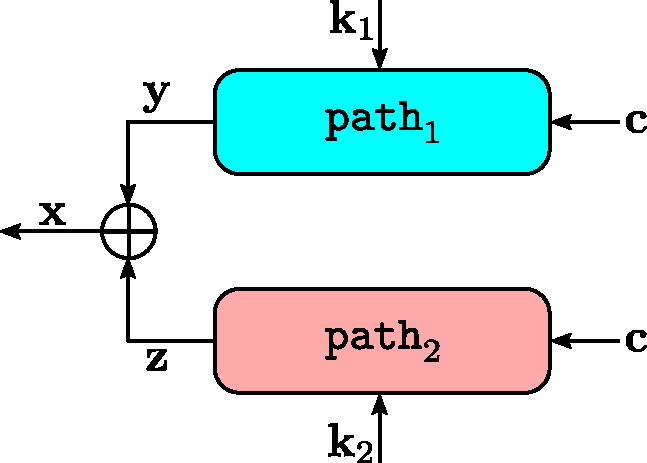
\includegraphics[width=0.9\textwidth]{./figures/mitm.pdf}
\[\visible<1->{\sum \bm{x} = 0} \visible<2->{\iff \sum \bm{y} = \sum \bm{z}}\]
\end{columns}
\end{frame}

\begin{frame}{Overall View of Our Key-Recovery Tool}
\begin{itemize}
	\item[1-] Assume that $\bm{x} = \bm{y} \oplus \bm{z}$ and $\sum \bm{x} = 0$
	\item[2-] For each path, i.e., $\bm{y}$, and $\bm{z}$:
	\begin{itemize}
	\item[-] Build the graph of dependencies: $\bm{y} = f(\bm{k}, \bm{c})$
	\item[-] Simplify the dependency graph: reform $f(\bm{k}, \bm{c})$ to $F(\bm{\tilde{k}} \oplus \bm{\tilde{c}})$
	\item[-] Use FFT to compute the list $[\sum \bm{y}\,|\, \bm{\tilde{k}} = 0, \ldots, 2^{|\bm{k}| - 1}]$
	\end{itemize}
	\item[3-] Compare the two lists to find candidates for the involved key bits
	\item[4-] Brute force the remaining keys to find the correct key
\end{itemize}
\end{frame}

\begin{frame}{Example: 3-Round Key Recovery}
	\centering
	\vspace{-0.4cm}
	\alt<2>{\color{white}}{\null\vspace{-0.65cm}}
	\warpround{24}{%
		\markbranches{5/12}
		\marksboxes{2/4/1}
	}
	
	\warpround{25}{%
		\markbranches{12/25,1/6}
		\marksboxes{0/0/31}
	}
	
	\warproundfinal{26}{%
		\markbranches{25/25,6/6,31/31}
		\marksboxes{12/24/24,15/30/30}
		\markoutputsnew[OUT]{25,6,31,24,30}
	}
	\pause
\end{frame}

\begin{frame}{Example: Dependency Graph}
	\centering
	\sparen
	\only<1>{%
		\begin{tikzpicture}[tree layout,
		grow=right,
		>=latex,
		sibling distance=.5cm, level distance=2cm,
		every edge quotes/.style={fill=white,draw,circle,inner sep=1pt},
		every label/.append style={gray,font=\footnotesize,below left},
		SBX/.style={>"S"},
		dup/.style={draw=red,dashed,thick},
		XOR/.style={circle,draw,inner sep=0pt}]
		\graph {
			X23i5/+ [XOR,label=$\X{23}{5}$] -> {
				X24i1/+ [SBX,XOR,label=$\X{24}{1}$] -> {
					X25i31/+ [SBX,XOR,label=$\X{25}{31}$] -> {
						Xout1/+ [XOR,label=$~$] -> {
							SY26i30/$\Y{26}{30}$ [SBX,OUT],
							Y26i31/$\Y{26}{31}$ [OUT],
						},
						K1i15/$\K{1}{15}$ [KEY],
					},
					Y26i6/$\Y{26}{6}$ [OUT],
					K0i0/$\K{0}{0}$ [KEY],
				},
				X25i25/+ [XOR,label=$\X{25}{25}$] -> {
					Xout2/+ [XOR,label=$~$] -> {
						SY26i24/$\Y{26}{24}$ [SBX,OUT],
						Y26i25/$\Y{26}{25}$ [OUT],
					},
					K1i12/$\K{1}{12}$ [KEY],
				},
				K1i2/$\K{1}{2}$ [KEY],
			}
		};
		\end{tikzpicture}%
	}
	\only<2>{%
		\begin{tikzpicture}[tree layout,
		grow=right,
		>=latex,
		sibling distance=.5cm, level distance=2cm,
		every edge quotes/.style={fill=white,draw,circle,inner sep=1pt},
		every label/.append style={gray,font=\footnotesize,below left},
		SBX/.style={>"S"},
		dup/.style={draw=red,dashed,thick},
		XOR/.style={circle,draw,inner sep=0pt}]
		\graph {
			X23i5/+ [XOR,label=$\X{23}{5}$] -> {
				X24i1/+ [SBX,XOR,label=$\X{24}{1}$] -> {
					X25i31/+ [SBX,XOR,label=$\X{25}{31}$] -> {
						SY26i30oplusY26i31/$S(\Y{26}{30})\oplus\Y{26}{31}$ [OUT],
						K1i15/$\K{1}{15}$ [KEY],
					},
					Y26i6/$\Y{26}{6}$ [OUT],
					K0i0/$\K{0}{0}$ [KEY],
				},
				X25i25/+ [XOR,label=$\X{25}{25}$] -> {
					SY26i24oplusY26i25/$S(\Y{26}{24})\oplus\Y{26}{25}$ [OUT],
					K1i12/$\K{1}{12}$ [KEY],
				},
				K1i2/$\K{1}{2}$ [KEY],
			}
		};
		\end{tikzpicture}%
	}
	\only<3>{%
		\begin{tikzpicture}[tree layout,
		grow=right,
		>=latex,
		sibling distance=.5cm, level distance=2cm,
		every edge quotes/.style={fill=white,draw,circle,inner sep=1pt},
		every label/.append style={gray,font=\footnotesize,below left},
		SBX/.style={>"S"},
		dup/.style={draw=red,dashed,thick},
		XOR/.style={circle,draw,inner sep=0pt}]
		\graph {
			X23i5/+ [XOR,label=$\X{23}{5}$] -> {
				X24i1/+ [SBX,XOR,label=$\X{24}{1}$] -> {
					X25i31/+ [SBX,XOR,label=$\X{25}{31}$] -> {
						SY26i30oplusY26i31/$S(\Y{26}{30})\oplus\Y{26}{31}$ [OUT],
						K1i15/$\K{1}{15}$ [KEY],
					},
					Y26i6/$\Y{26}{6}$ [OUT],
					K0i0/$\K{0}{0}$ [KEY],
				},
				K1i2oplusK1i12/$\K{1}{2}\oplus\K{1}{12}$ [KEY],
				SY26i24oplusY26i25/$S(\Y{26}{24})\oplus\Y{26}{25}$ [OUT],
			}
		};
	\end{tikzpicture}%
	}
\end{frame}

\begin{frame}{Summary of Our Result}
\begin{table}[h!]
	\centering
	\label{tab:summary_keyrecovery}
	\newcommand{\ph}{\phantom{.00}}
	\resizebox{0.8\textwidth}{!}{
	\begin{tabular}{@{}lccclrl@{}}
		\toprule
		\#R    & Data             & Time         & Memory             & Attack           & Reference\\
		\midrule
		\bf 32 &     $2^{127\ph}$ & $2^{127\ph}$ & $2^{108\ph}$       & Integral         & This paper\\
		21 &     $2^{124\ph}$ & -            & -                      & Integral         & \cite{sacrypt_BanikBIKLMSSS20}\\
		\midrule
        18 &     $2^{104.62}$ & -            & -                      & Differential     & \cite{journals_istr_TehB22}\\
		21 &     -            & -            & -                      & Impossible diff. &  \cite{sacrypt_BanikBIKLMSSS20}\\
		21 &     $2^{113\ph}$ & $2^{113\ph}$ & $2^{72\phantom{0.00}}$ & Differential     & \cite{conf_space_KumarY21}\\
		23 &     $2^{106.62}$ & $2^{106.62}$ & $2^{106.62}$           & Differential     &  \cite{journals_istr_TehB22}\\
		%\midrule
		24 &     $2^{126.06}$ & $2^{125.18}$ & $2^{127.06}$           &  Rectangle       & \cite{journals_istr_TehB22}\\
		\bottomrule
	\end{tabular}}
\end{table}
\end{frame}

\section{Conclusion}
\sectionheader[\huge\color{tug}\faClockO]{Conclusion}
\begin{frame}{Contributions}
\begin{itemize}
\small
\item[\faCheckCircle] We provided a SAT model for integral analysis based on Monomial prediction
\item[\faCheckCircle] Our modeling is generic and can be applied to other (binary field) block ciphers
\item[\faCheckCircle] We proposed a tool for key-recovery taking the FFT technique into account
\item[\faDiamond] Overall, we improved the integral attack of \cipher{WARP} by \textbf{\textcolor{red}{11}} rounds
\end{itemize}
\begin{center}

{\large Thanks for your attention!}

\vspace{0.5cm}
\url{https://github.com/hadipourh/mpt}
\end{center}
\end{frame}

















%%%%%%%%%%%%%%%%%%%%%%%%%%%%%%%%%%%%%%%%%%%%%%%%%%%%%%%%%%%%%%%%%%%%%%%%%%%%

\begin{frame}[allowframebreaks]{Bibliography}
  \printbibliography
\end{frame}

\begin{filecontents*}[overwrite]{\jobname.bib}

@inproceedings{monomial_prediction_asiacrypt_HuSW020,
  author    = {Kai Hu and
               Siwei Sun and
               Meiqin Wang and
               Qingju Wang},
  title     = {An Algebraic Formulation of the Division Property: Revisiting Degree
               Evaluations, Cube Attacks, and Key-Independent Sums},
  booktitle = {{ASIACRYPT} 2020},
  series    = {LNCS},
  volume    = {12491},
  pages     = {446--476},
  publisher = {Springer},
  year      = {2020},
  doi       = {10.1007/978-3-030-64837-4_15},
}

@inproceedings{sacrypt_BanikBIKLMSSS20,
  author    = {Subhadeep Banik and
               Zhenzhen Bao and
               Takanori Isobe and
               Hiroyasu Kubo and
               Fukang Liu and
               Kazuhiko Minematsu and
               Kosei Sakamoto and
               Nao Shibata and
               Maki Shigeri},
  title     = {{WARP}: Revisiting {GFN} for Lightweight 128-Bit Block Cipher},
  booktitle = {{SAC} 2020},
  series    = {LNCS},
  volume    = {12804},
  pages     = {535--564},
  publisher = {Springer},
  year      = {2020},
  doi       = {10.1007/978-3-030-81652-0_21}
}

@incollection{hod_discrete_derivatives_lai1994higher,
  author    = {Lai, Xuejia},
  title     = {Higher order derivatives and differential cryptanalysis},
  booktitle = {Communications and cryptography},
  pages     = {227--233},
  year      = {1994},
  publisher = {Springer}
}

@inproceedings{square_fse_DaemenKR97,
  author    = {Joan Daemen and
               Lars R. Knudsen and
               Vincent Rijmen},
  title     = {The Block Cipher {Square}},
  booktitle = {{FSE} 1997},
  series    = {LNCS},
  volume    = {1267},
  pages     = {149--165},
  publisher = {Springer},
  year      = {1997},
  doi       = {10.1007/BFb0052343},
}

@inproceedings{cansTodoA14,
  author    = {Yosuke Todo and
               Kazumaro Aoki},
  title     = {{FFT} Key Recovery for Integral Attack},
  booktitle = {{CANS} 2014},
  series    = {LNCS},
  volume    = {8813},
  pages     = {64--81},
  publisher = {Springer},
  year      = {2014},
  doi       = {10.1007/978-3-319-12280-9_5},
}

@inproceedings{sacryptSasaki012,
  author    = {Yu Sasaki and
               Lei Wang},
  title     = {Meet-in-the-Middle Technique for Integral Attacks against {Feistel}
               Ciphers},
  booktitle = {SAC 2012},
  series    = {LNCS},
  volume    = {7707},
  pages     = {234--251},
  publisher = {Springer},
  year      = {2012},
  doi       = {10.1007/978-3-642-35999-6_16},
}

@article{journals_istr_TehB22,
	author    = {Je Sen Teh and
		Alex Biryukov},
	title     = {Differential cryptanalysis of {WARP}},
	journal   = {J. Inf. Secur. Appl.},
	volume    = {70},
	pages     = {103316},
	year      = {2022},
	url       = {https://doi.org/10.1016/j.jisa.2022.103316},
	doi       = {10.1016/j.jisa.2022.103316}
}

@inproceedings{conf_space_KumarY21,
	author    = {Manoj Kumar and
		Tarun Yadav},
	title     = {{MILP} Based Differential Attack on Round Reduced {WARP}},
	booktitle = {{SPACE} 2021},
	series    = {LNCS},
	volume    = {13162},
	pages     = {42--59},
	publisher = {Springer},
	year      = {2021},
	doi       = {10.1007/978-3-030-95085-9_3},
}
\end{filecontents*}

\end{document}
